\section{Путь пользователя}

\subsection{Карта сценариев}

Все операции используют один понятный цикл: сотрудник открывает назначенное задание, сканирует товар, проверяет данные, подтверждает результат и получает итог выполнения.

\begin{center}
\small
Выбор задания $\longrightarrow$ Накладная $\longrightarrow$ Сканирование $\longrightarrow$ Подтверждение $\longrightarrow$ Итог
\end{center}

\subsection{C01. Приемка}\label{scenario:receiving}


\begin{tabularx}{\textwidth}{L{42mm}Y}
\toprule
\textbf{Что описать} & \textbf{Сценарий приемки} \\
\midrule
Экраны & Главный экран (приемка товаров) -> Выбор накладной -> сканирование EAN-13 на коробках от поставщика -> подтверждение количества коробок -> завершение приемки фотография накладной \\
Результат & Принятые позиции фиксируются в задании; для непринятых или не соответствующих заданию товаров указывается расхождение. \\
\bottomrule
\end{tabularx}

\subsubsection{Экраны пути пользователя}

\begin{center}
\begin{tabular}{@{}ccc@{}}
\phonescreen{1}{assets/receiving/01-main.png}{Главный экран} &
\phonescreen{2}{assets/receiving/02-note-selection.png}{Выбор накладной} &
\phonescreen{3}{assets/receiving/03-receiving-task.png}{Задание на приёмку} \\
[5mm]
\phonescreen{4}{assets/receiving/04-box-confirmed.png}{Коробка принята} &
\phonescreen{5}{assets/receiving/05-box-review.png}{Проверка коробки} &
\phonescreen{6}{assets/receiving/06-discrepancy.png}{Фиксация расхождения, если было отсанировано меньше коробок чем в накладной} \\
\end{tabular}
\end{center}

\subsubsection{Экраны пути пользователя (продолжение)}

\begin{center}
\begin{tabular}{@{}ccc@{}}
\phonescreen{7}{assets/receiving/07-receiving-result.png}{Итог приёмки} &
\phonescreen{8}{assets/receiving/08-receipt-photo.png}{Фотографирование накладной} &
\phonescreen{9}{assets/receiving/09-receiving-result-with-photo.png}{Накладная прикреплена} \\
\end{tabular}
\end{center}

\subsubsection{Описание сценария}

Этап «Приёмка» предназначен для подтверждения фактически полученного товара по заранее созданному заданию на приёмку.

\begin{enumerate}
    \item На главном экране сотрудник открывает раздел «Приёмка». В списке отображаются доступные задания, ожидающие обработки.
    \item Сотрудник выбирает нужное задание на приёмку. Перед началом работы он сверяет номер задания, поставщика и сопроводительные документы с прибывшей поставкой.
    \item После открытия задания сотрудник поочерёдно сканирует штрихкоды всех коробок, входящих в поставку. Каждая коробка сканируется отдельно.
    \item После каждого сканирования приложение проверяет штрихкод и фиксирует коробку в текущем задании. На экране обновляется ход приёмки: количество отсканированных коробок, оставшиеся позиции и возможные расхождения.
    \item Если штрихкод не распознан, коробка отсутствует в задании или была отсканирована повторно, приложение сообщает об этом сотруднику. Проблемная ситуация фиксируется в отчёте о приёмке: сотрудник добавляет комментарий с причиной, а приложение не изменяет количество повторно.
    \item Сотрудник продолжает сканирование до обработки всех коробок, указанных в задании. Перед завершением он убеждается, что необработанные позиции и неподтверждённые расхождения отсутствуют.
    \item После успешного сканирования поставки сотрудник выбирает действие «Закрыть приёмку». Система сохраняет результаты, закрывает задание и фиксирует факт приёмки товара.
    \item В завершение сотрудник прикрепляет к отчёту фотографию подписанной накладной или другого подтверждающего документа. Фотография сохраняется в отчёте о приёмке и после завершения доступна при его просмотре.
\end{enumerate}

После закрытия приёмки товар считается принятым и готовым к следующей складской операции --- размещению в зоне хранения.

\subsection{C02. Размещение}\label{scenario:placement}

\subsubsection{Экраны пути пользователя}

\begin{center}
\begin{tabular}{@{}ccc@{}}
\phonescreen{1}{assets/placement/01-scan-product.jpeg}{Задание: отсканировать товар} &
\phonescreen{2}{assets/placement/02-scan-location.jpeg}{Товар распознан: отсканировать ячейку} &
\phonescreen{3}{assets/placement/03-confirm-placement.jpeg}{Ячейка совпадает: подтвердить размещение} \\
[5mm]
\phonescreen{4}{assets/placement/04-position-placed.jpeg}{Позиция размещена: сканировать следующий товар} &
\phonescreen{5}{assets/placement/05-placement-result.jpeg}{Все позиции размещены: вернуться к операциям} \\
\end{tabular}
\end{center}

\subsubsection{Описание сценария}

Этап «Размещение» предназначен для размещения товаров на полках в назначенных ячейках. К выполнению операции сотрудник приступает после завершения приёмки, когда товары становятся доступны для размещения.

\begin{enumerate}
    \item На главном экране сотрудник открывает раздел «Размещение» и выбирает нужное задание. В задании отображаются товары, которые нужно разложить по ячейкам, и ход выполнения: сколько товаров уже размещено и сколько осталось.
    \item Сотрудник берёт первый товар и сканирует его штрихкод EAN-13. Приложение находит товар в локальном каталоге и проверяет, что он входит в выбранное задание и ещё не был размещён.
    \item После успешной проверки приложение показывает ячейку, в которую нужно положить товар. Сотрудник переносит товар к этой ячейке и кладёт его на полку.
    \item Сотрудник сканирует штрихкод ячейки. Приложение сопоставляет отсканированную ячейку с ячейкой, назначенной для данного товара, и сообщает о совпадении.
    \item Сотрудник проверяет название товара и ячейку на экране, затем нажимает «Подтвердить размещение». Только после этого приложение фиксирует товар на полке и увеличивает счётчик выполненных товаров на один.
    \item Приложение показывает, что позиция размещена, и переходит к следующему неразмещённому товару. Сотрудник повторяет последовательность «сканировать товар -> сканировать ячейку -> подтвердить размещение» до тех пор, пока все товары задания не окажутся на своих местах.
    \item Если отсканирован другой товар, уже размещённый товар или неверная ячейка, приложение сообщает о несоответствии и не изменяет данные. Сотрудник проверяет маркировку и повторяет сканирование корректного товара или ячейки.
    \item Когда все товары задания размещены, приложение показывает итог операции: все товары находятся на назначенных полках, задание завершено, а сотрудник может вернуться к выбору операций.
\end{enumerate}

После завершения операции каждый товар задания считается размещённым в назначенной ячейке и доступным для дальнейших складских операций.

\begin{tabularx}{\textwidth}{L{42mm}Y}
\toprule
\textbf{Что описать} & \textbf{Сценарий размещения} \\
\midrule
Экраны & Задание: сканирование товара -> товар распознан: сканирование ячейки -> ячейка совпадает: подтверждение -> позиция размещена: следующий товар -> итог. \\
Действия сотрудника & Для каждого товара сканирует товар, сканирует назначенную ячейку, проверяет совпадение и подтверждает размещение. Повторяет действия, пока все товары задания не будут размещены. \\
Результат & После подтверждения корректной ячейки приложение фиксирует товар на этой полке, сохраняет ход выполнения на устройстве и по завершении предлагает вернуться к выбору операций. \\
\bottomrule
\end{tabularx}

\subsection{C03. Сканирование штрихкода}\label{scenario:barcode-scanning}

\begin{tabularx}{\textwidth}{L{42mm}Y}
\toprule
\textbf{Что описать} & \textbf{Сценарий сканирования штрихкода} \\
\midrule
Экраны & Экран сканирования камерой -> проверка кода -> возврат к заданию с результатом; альтернативный путь: ручной ввод EAN-13 -> проверка кода -> возврат к заданию с результатом. \\
Способы ввода & Камера является основным способом. Ручной ввод используется, если этикетка повреждена, камера недоступна или штрихкод невозможно считать. Оба способа проходят одинаковую проверку. \\
Результат & Код либо принимается для просмотра и последующего подтверждения операции, либо отклоняется с понятной причиной. Само сканирование или ручной ввод не изменяют остатки, количество и результат задания. \\
\bottomrule
\end{tabularx}

\subsubsection{Пример экранов при сканировании}


\begin{center}
\begin{tabular}{@{}cc@{}}
\phonescreen{1}{assets/scanning/01-camera-scan.png}{Сканирование камерой} &
\phonescreen{2}{assets/scanning/02-manual-entry.png}{Ручной ввод штрихкода} \\
\end{tabular}
\end{center}

\subsubsection{Описание сценария работы сканера}

Экран сканирования открывается из выбранного задания по кнопке «Сканировать». Он получает контекст текущего задания: вид операции, ожидаемый товар, требуемое количество, исходную и целевую ячейки при их наличии.

\begin{enumerate}
    \item При открытии основного экрана запускается камера устройства. Сотрудник видит изображение с камеры, рамку для штрихкода. На экране доступны действия «Отмена» и переход к ручному вводу данных штрих кода.
    \item Сотрудник размещает этикетку коробки в рамке. После распознавания камера приостанавливается, чтобы один и тот же штрихкод не был считан несколько раз подряд. Приложение подаёт короткий звуковой или вибрационный сигнал и начинает проверку кода.
    \item Считанное значение очищается от пробелов по краям и проверяется как EAN-13: оно должно состоять из 13 цифр и иметь корректную контрольную цифру. Коды других форматов, неполные коды и коды с ошибочной контрольной цифрой не принимаются.
    \item Для корректного EAN-13 приложение ищет конкретный товар в локальном каталоге устройства, затем проверяет, соответствует ли товар текущему заданию и доступен ли он для выбранной операции. До завершения этой проверки сотруднику не показывается подтверждение операции.
    \item Если камера не может считать этикетку, сотрудник выбирает ручной ввод. На отдельном экране он вводит 13 цифр EAN-13 и нажимает «Проверить». Ручной код проходит ровно те же проверки, что и считанный камерой; ручной ввод не является способом обойти проверку товара или задания.
    \item Сотрудник может отменить сканирование или ручной ввод в любой момент. Приложение возвращает его в задание без сохранения кода и без изменения данных.
\end{enumerate}

\clearpage
\begin{landscape}
\subsubsection{Блок-схема обработки результата сканирования}

Проверки выполняются до показа карточки товара и до подтверждения операции.

\begin{center}
  \vspace*{\fill}
  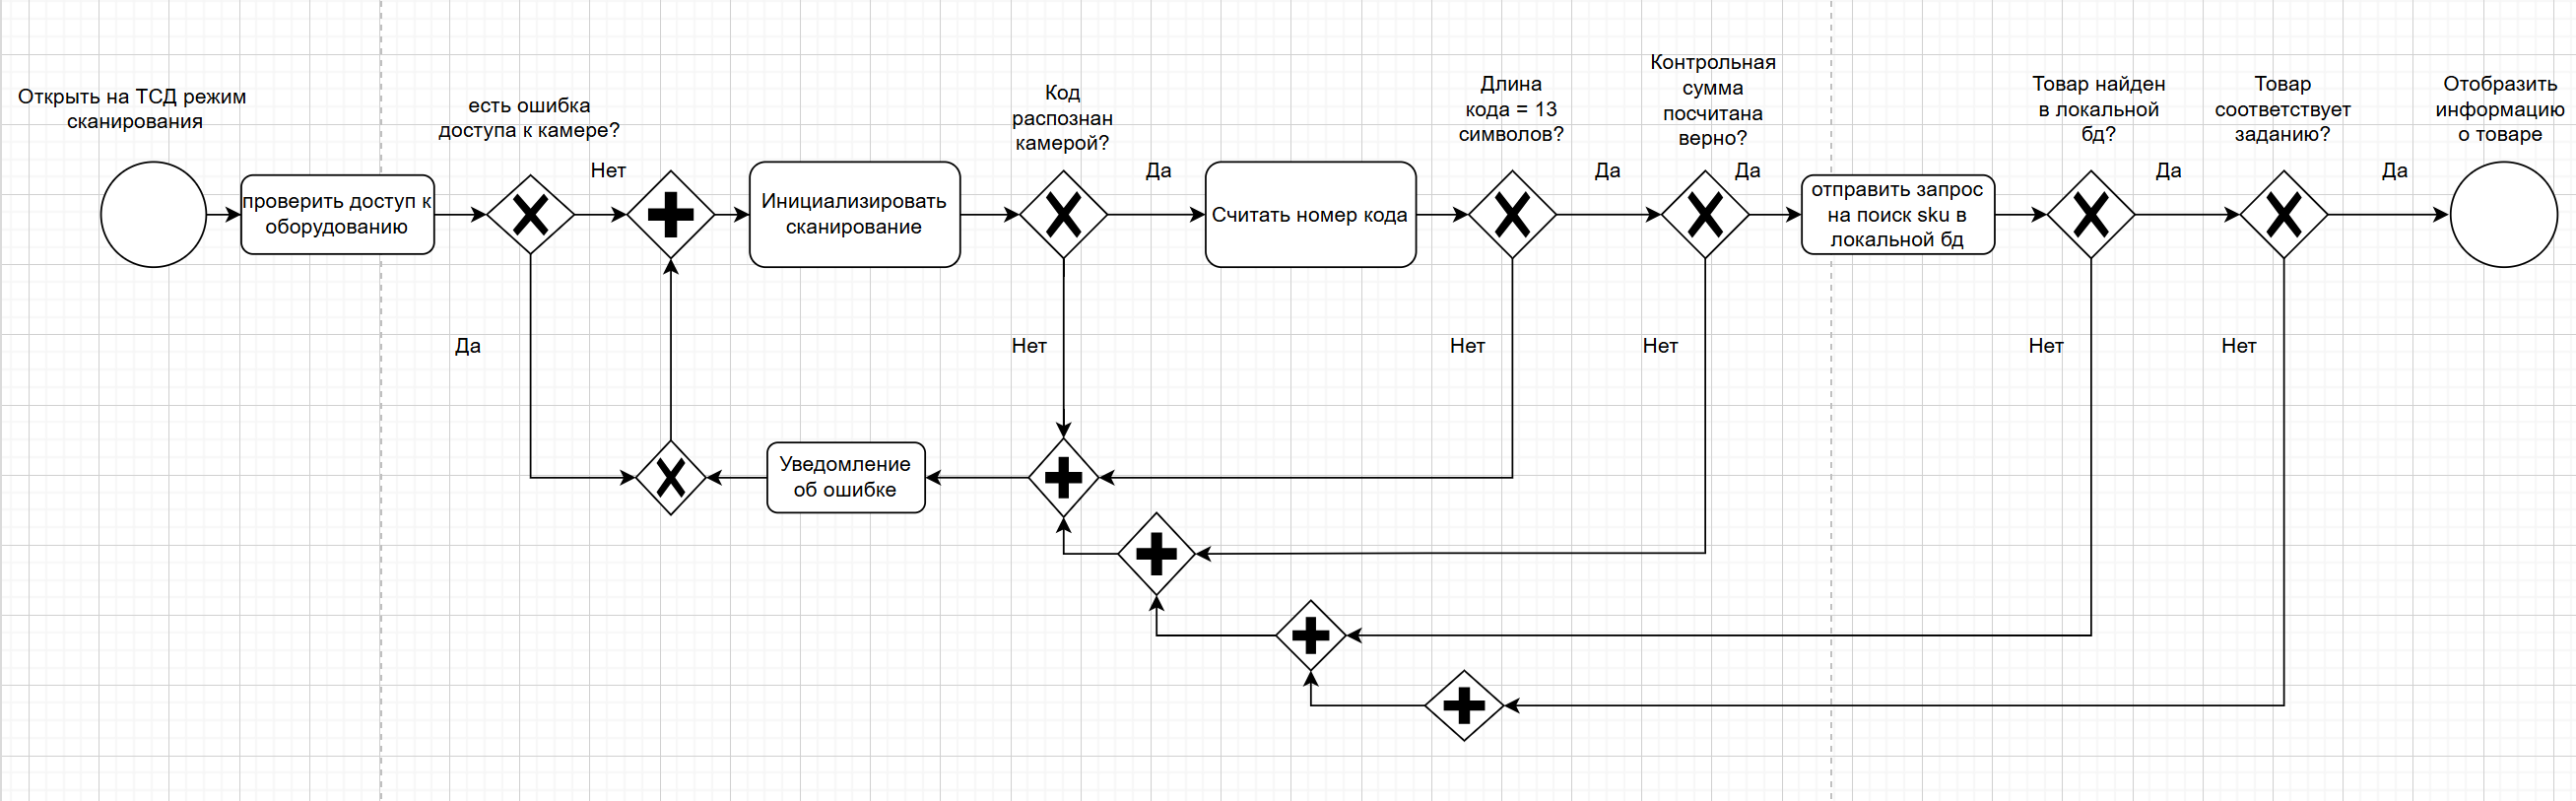
\includegraphics[width=\linewidth,keepaspectratio]{assets/scanning/scanning-result-processing-flow.png}
  \par\smallskip
  \refstepcounter{figure}\small\textbf{\figurename~\thefigure~---} Процесс сканирования и обработки результата
  \label{fig:scanning-result-processing}
  \vspace*{\fill}
\end{center}
\end{landscape}
\clearpage

\subsubsection{Обработка сложных ситуаций}

\begin{longtable}{L{44mm}L{112mm}}
\toprule
\textbf{Ситуация} & \textbf{Поведение приложения и действие сотрудника} \\
\midrule
\endfirsthead
\toprule
\textbf{Ситуация} & \textbf{Поведение приложения и действие сотрудника} \\
\midrule
\endhead
Штрихкод не распознан камерой & На экране выводится сообщение «Не удалось считать штрихкод. Наведите камеру ещё раз». Данные не изменяются, камера остаётся доступной для повторной попытки; сотрудник может переключиться на ручной ввод. \\
Распознан неподдерживаемый формат & Приложение сообщает «Нужен штрихкод EAN-13». Код не передаётся в задание, камера возобновляет работу после сообщения. \\
Некорректный EAN-13 & При ручном вводе поле принимает только цифры; при нажатии «Проверить» приложение сообщает о необходимости ввести 13 цифр с верной контрольной цифрой. При сканировании камера возобновляет работу. \\
Товар не найден в каталоге & Отображается сообщение «Товар не найден в локальном каталоге». Код не принимается, количество и остатки не меняются. Сотрудник проверяет этикетку, повторяет сканирование или передаёт ситуацию ответственному сотруднику. \\
Товар не соответствует заданию & Приложение сообщает, что отсканирован неподходящий товар, и показывает ожидаемый товар. Подтверждение операции недоступно до сканирования корректной коробки. \\
Коробка отсканирована повторно & Если коробка уже была принята или размещена в рамках текущего задания, приложение выводит сообщение «Коробка уже обработана». Повторное сканирование не увеличивает количество, не меняет остатки и не создаёт вторую запись операции; сотрудник сканирует следующую коробку. \\
Задание уже завершено & Приложение сообщает «Задание уже выполнено» и не принимает код. Сотрудник возвращается к списку заданий и выбирает актуальное задание. \\
Недостаточно товара для операции & Приложение сообщает, что товара в исходной ячейке недостаточно, и не позволяет подтвердить действие. Сотрудник проверяет предыдущее размещение или обращается к ответственному сотруднику. \\
Нет разрешения на камеру & Экран объясняет, что для сканирования нужен доступ к камере, и предлагает кнопки «Повторить» и «Открыть настройки Android». До выдачи разрешения доступен ручной ввод и отмена. \\
Камера занята или недоступна & Отображается понятное сообщение с рекомендацией закрыть другое приложение, использующее камеру. Сотрудник может повторить запуск камеры, перейти к ручному вводу или отменить действие. \\
\bottomrule
\end{longtable}
